%----------------------------------------------------------------------------------------
%	PACKAGES AND OTHER DOCUMENT CONFIGURATIONS
%----------------------------------------------------------------------------------------

\documentclass[12pt]{article}
\usepackage{graphicx}
\usepackage[utf8]{inputenc}  
\usepackage[T1]{fontenc} 
\usepackage[top=2cm,bottom=2cm,left=1.3cm,right=1cm,asymmetric]{geometry}

\usepackage{amsfonts}
\usepackage{graphicx}
\usepackage{fancyhdr}
\usepackage{array,multirow,makecell}
\usepackage{amsmath}

\usepackage{cancel}
\usepackage{subfig}
\usepackage{wrapfig}

\newcommand\independent{\protect\mathpalette{\protect\independenT}{\perp}}
\def\independenT#1#2{\mathrel{\rlap{$#1#2$}\mkern2mu{#1#2}}}

\setcellgapes{1pt}
\makegapedcells
\newcolumntype{R}[1]{>{\raggedleft\arraybackslash }b{#1}}
\newcolumntype{L}[1]{>{\raggedright\arraybackslash }b{#1}}
\newcolumntype{C}[1]{>{\centering\arraybackslash }b{#1}}

\pagestyle{fancy}
\renewcommand{\footrulewidth}{1pt}
\fancyhead[R]{\textit{Master MVA : Graphical models}}
\fancyfoot[L]{\textit{}}
%\usepackage{unicode-math}
%\setmathfont{XITS Math}
%\setmathfont[version=setB,StylisticSet=1]{XITS Math}


%\geometry{hmargin=1.5cm,vmargin=2cm}   

\begin{document}


\section*{Sammy Khalife \& Matias Tailanian}
\subsubsection*{29/10/2014}
\subsubsection*{Assignment 2}
\section*{1 Distributions factorizing in a graph} 
\subsection*{a.}
- Given the definition of $p \in L(G)$, we have for any x :
\begin{eqnarray*}
p(x) & = & \prod_{k=1}^{n}p(x_{k}|x_{\pi_{k}})\\
& = &  \prod \limits^n_{\substack{k=1 \\ k \neq i k \neq j} }p(x_{k}|x_{\pi_{k}}) \; p(x_{i}|x_{\pi_{i}})p(x_{j}|x_{\pi_{i}},x_{i})
\end{eqnarray*}
Since by assumption, $\pi_{j}=\pi_{i} \cup {i}$: $p(x_j|x_{\pi_j})=p(x_j|x_{\pi_{i\cup i}})=p(x_j|x_{\pi_i},x_i)$.~\\
Thanks to the Bayes formula applied to $p(x_{j}|x_{\pi_{i}}, x_{i})$ :
\begin{eqnarray*}
p(x) & = & \prod \limits_{\substack{k=1 \\ k \neq i k \neq j} } p(x_{k}|x_{\pi_{k}})        
\cancel {p(x_{i}|x_{\pi_{i}})}
p(x_{i}|x_{\pi_{i}},x_{j})\frac{p(x_{j}|x_{\pi_{i}})}{\cancel{p(x_{i}|x_{\pi_{i}})}}\\
& = &  \prod \limits_{\substack{k=1 \\ k \neq i k \neq j} } p(x_{k}|x_{\pi_{k}})p(x_{i}|x_{\pi_{i}},x_{j})p(x_{j}|x_{\pi_{i}})
\end{eqnarray*}
This last equality is saying that $p$ is factorizing in $G^{'}=(V,E^{'})$, with $E^{'} = (E \setminus \{ i \mapsto j \}\cup\{j\mapsto i\})$. ~\\
Then $L(G) \subset L(G')$.~\\
By going back in the equalities, we actually have $L(G^{'}) \subset L(G)$.
Hence, $L(G)=L(G^{'})$.
~\\
~\\
- As $G$ is a directed tree, it's also a \emph{graph}, so $p(x)$ factorizes in $G$:
$$p(x) = \prod^n_{i=1}p(x_i|x_{\pi_i})$$
As $G$ is a directed tree with no \emph{v-structures}, it has the same quantity of \emph{edges} as \emph{clicks}: $n-1$. Furthermore each click has two elements, i.e. sets parent-children. Dividing and multiplying the previous expression by $n-1$, and defining $\psi_{c} = (n-1)f(x_c,x_{\pi_c})$ (without ambiguity because there is only one node having no parents in the clique) and $Z=n-1$ (the number of clicks), we obtain:
$$p(x) = \frac{1}{Z}\prod_{c\in \mathcal{C}}\psi_c(x_c)$$
where $\mathcal{C}$ is the set of clicks of $G$. This expression corresponds to a factorization in the symetrized graph $G^\prime$ of $G$, which has $Z=n-1$ clicks of cardinal $2$, $\{x_k, x_{\pi_k}\}$, proving: $\mathcal{L}(G)\subseteq \mathcal{L}(G^\prime)$.
~\\
~\\
In the other hand, as $E^\prime \subseteq E$, by \textbf{proposition 4.4}: $\mathcal{L}(G^\prime)\subseteq \mathcal{L}(G)$.
Finally, $$\boxed{\mathcal{L}(G) = \mathcal{L}(G^\prime)}$$
%TODO: doubt. (n-1) inside the prod?

\subsection*{b.}

\section*{2 d-separation}
\subsection*{a.}
By the definition of \textbf{moralized graph}, we can construct $\mathbf{G_M(V,E_M)}$ by first constructing the \textbf{symmetrized graph} $\mathbf{\tilde{G}}$ of $\mathbf{G(V,E)}$, and then adding edges such that for all $v\in V,\ \pi_v$ is a click. By definition, $\mathbf{E}\subset \mathbf{E_M}$. Therefore, given that $S$ separates $A$ and $B$ in $\mathbf{G_M}$, $A$ and $B$ are d-separated in $\mathbf{G}$.

\subsection*{b.}
No. Counterexample shown in Figure \ref{fig:ex2_dags}.
\begin{figure} [h!]
\centering
  \subfloat[Simple DAG]{\label{fig:dagSimple} 
  		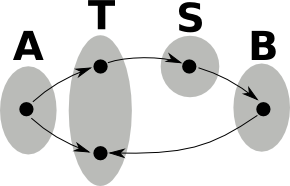
\includegraphics[width=.4\textwidth]{./pics/dagSimple.png}} \hfill 
  \subfloat[Complex DAG]{\label{fig:dagComplex} 
  		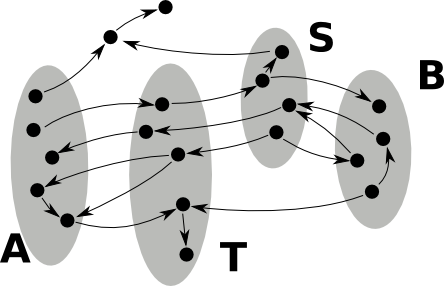
\includegraphics[width=.5\textwidth]{./pics/dagComplex.png}} \\
  \caption{Counterexample}
  \label{fig:ex2_dags}
\end{figure}

\subsection*{c.}
\begin{wrapfigure}{r}{0.4\textwidth}
	\vspace{-20pt}
	\begin{center}
		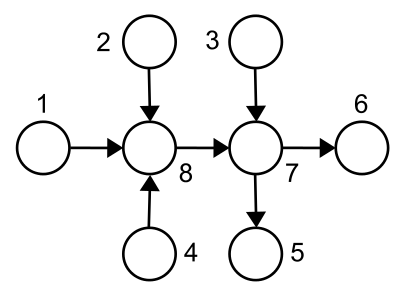
\includegraphics[width=0.3\textwidth]{./pics/ex2c.png}
	\end{center}
	\vspace{-20pt}
	\caption{Graph $G$}
	\label{fig:ex2c}
\end{wrapfigure}
Given the graph shown in Figure \ref{fig:ex2c}, we consider the following statements:
\begin{enumerate}
	\item $X_{\{1,2\}}\independent X_4|X_3$
	\item $X_{\{1,2\}}\independent X_4|X_5$
	\item $X_1\independent X_6|X_{\{2,4,7\}}$
\end{enumerate}
As nodes (1) and (4) forms a v-structure with node (8), they are not independent unless (8) is in the given set (unless (8) is observed). The same situation occurs between nodes (2) and (4) (they form a v-structure with node (8)). Therefore, statements 1. and 2. are FALSE. In the other hand, statement 3. is TRUE because the only chain from (1) to (8) is blocked by (7).

\section*{Implementation - Gaussian Mixtures}
\subsection*{a.}
\begin{figure}[h!]
	\centering 
	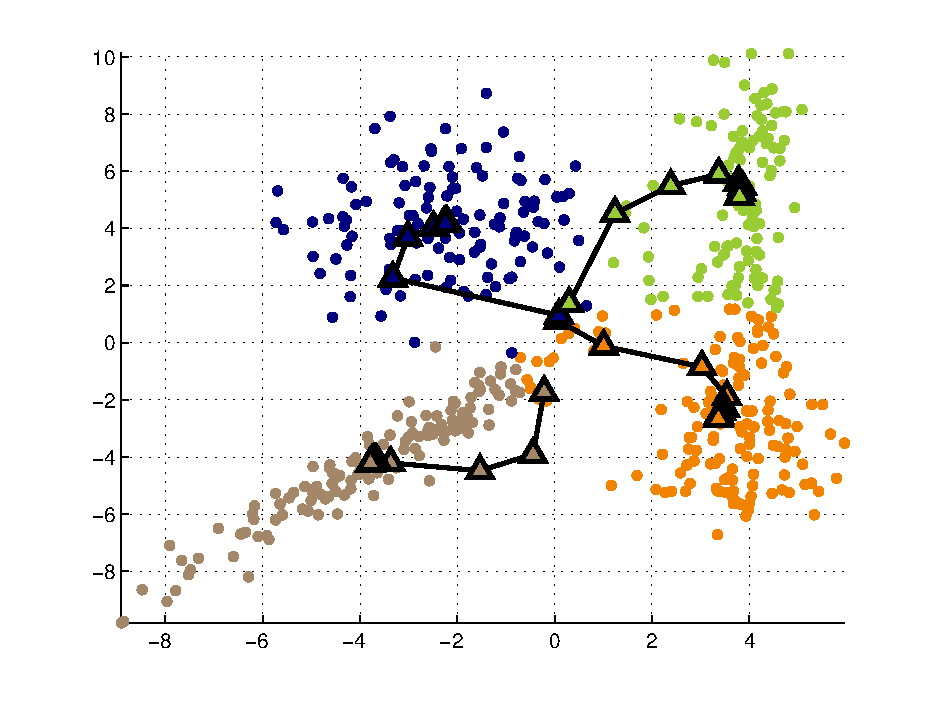
\includegraphics[width=.8\textwidth]{./pics/3a.pdf}
	\caption{K-Means algorithm output}
	\label{fig:3a}
\end{figure}

\end{document}